\chapter{Direkte Fernlokalisierung mit 802.11}
\label{ch:phase2}
Bei der direkten Fernlokalisierung wird die Messgröße auf den Basisstationen gemessen.
Die Ortungsinformation wird dann implizit durch versenden der gemessenen Werte an den Ortungsserver übermittelt.
Dieser berechnet dann aus den gesammelten Werten die Position der mobilen Einheit.
Eine Lösung zur direkten Fernlokalisierung muss deshalb nicht mit einem Access Point assoziiert sein.
APs versenden die gemessenen Werte jedoch nicht automatisch an den Ortungsserver. 
Sollen also die APs des WLAN-Netzwerks auch als Basisstationen verwendet werden, muss ihre Software es erlauben den in der Analyse als Messgröße ausgewählten Received Signal Strength Index bestimmter Pakete abzurufen.

%TODO Tags weg
\section{RADAR Implementierung}
Eine mobile Einheit mit RADAR versendet alle 0,25 Sekunden ein 6 Byte langes UDP-Paket, der RSSI der Übertragung wird dann auf dem AP gemessen.
Das Sendeintervall wurde so kurz gewählt, um spontane Schwankungen im RSSI durch mehrfache Messung zu glätten und sich bewegende Personen möglichst genau zu erfassen.
Für eine Bereichsortung reicht ein wesentlich längeres Sendeintervall, es wird erneut ein Intervall von fünf Sekunden gewählt, in dem sich ein Mitarbeiter maximal 42 Meter bewegt. 
Tabelle \ref{table:radarconsumption} zeigt den mit dem TM103 gemessenen Verbrauch der Implementierung für mobile Einheiten mit RADAR jeweils in Arduino und C, mit unterschiedlich langen Sendeintervallen mit und ohne manuellen \texttt{light\_sleep}.

\begin{table}[h]
	\centering
	\caption{Energieverbrauch RADAR-artiger mobiler Einheiten}
	\label{table:radarconsumption}
	\begin{tabular}{p{3cm}|p{2.2cm}|p{1.5cm}|p{2cm}|p{2cm}|p{2cm}}
		SDK & manueller \texttt{light\_sleep} & Sende"-intervall in s & Versuchs-dauer in Stunden & Gesamt-verbrauch in mAh & $\varnothing$ Verbrauch in mA \\
		\hline
		Arduino Core & Nein & 0,25 & 2 & 80 & 40 \\
		Arduino Core & Ja & 0,25 & 3 & 119 & 39,66 \\
		Arduino Core & Nein & 5 & 3 & 28 & 9,33 \\
		Arduino Core & Ja & 5 & 3 & 23 & 7,66 \\
		ESP Open SDK & Nein & 0,25 & 1 & 40 & 40 \\
		ESP Open SDK & Ja & 0,25 & 1 & 38 & 38 \\
		ESP Open SDK & Nein & 5 & 2 & 12 & 6 \\
		ESP Open SDK & Ja & 5 & 2 & 10 & 5 \\
	\end{tabular}
\end{table}

Der Energieverbrauch einer Lösung die vier Pakete pro Sekunde sendet ist wie erwartet hoch.
Die Implementierungen mit der ESP Open SDK und manuellem \texttt{light\_sleep} unterscheiden sich ausschließlich im Sendeintervall, dies verändert den Energieverbrauch jedoch stark.
Die dort besprochenen Optimierungen (nur bei AP-Wechsel senden) können auch für die RADAR Implementierung verwendet werden, das RADAR-artige mobile Einheit ist dann aber in seiner Implementierung bis auf den Inhalt des UDP-Pakets identisch mit dem der mobilen Einheiten für Bereichsortung.
Der Energieverbrauch sollte sich somit kaum unterscheiden und ein System mit RADAR-artigen mobilen Einheiten benötigt Veränderungen der Software der APs, ein System mit mobilen Einheiten für Bereichsortung ist deshalb vorzuziehen. 
Die Implementierung in C mit einem Sendeintervall von fünf Sekunden wird in Abschnitt \ref{ch:phase2:sec:powerradar} genauer untersucht.

\section{Anpassungen für Bereichsortung}
\label{ch:phase2:sec:anpassungbereich}
RADAR versendet immer noch UDP Pakete und arbeitet damit auf Schicht vier (Transport) des OSI-Modells und muss im Netzwerk authentifiziert und mit einem Access Point assoziiert sein.
Das ist für eine direkte Fernlokalisierung aber nicht notwendig, der RSSI wird auf Schicht eins (PHY) gemessen.
Grundsätzlich kann aufgrund der möglichen Änderungen am AP ein beliebiges Paket mit einer speziellen Kennung versendet und vom AP als Positionsmitteilung der mobilen Einheit erkannt werden. \\
Ein Sendevorgang, der nur Schicht eins nutzt hat einen geringeren Energieverbrauch, da er nur senden und nie empfangen muss.
Ein solcher Sendevorgang könnte aber die Funktion des Netzwerks beeinträchtigen und stellt nicht sicher, dass die eigene Übertragung nicht durch andere Übertragungen gestört wurde.
Es sollte deshalb nicht auf Schicht eins gearbeitet werden.\\
Stattdessen sollte Schicht zwei (MAC) des OSI-Modells verwendet werden. 
Da 802.11 für den Mediumszugriff eine Kollisionsvermeidung (CSMA/CA) verwendet wird, muss die mobile Einheit vor dem Senden das Medium belauschen, um zu bestimmen ob es belegt ist.
Der Energieverbrauch ist somit pro Sendevorgang höher als bei einer Lösung auf Schicht eins, stellt dafür aber die Verfügbarkeit des Mediums (der Frequenz) für die übrigen Teilnehmer sicher. \\
Um die Änderungen an der Software des AP gering zu halten wurde der Probe Request als zu sendender Frame gewählt.
Es handelt sich dabei um einen Management Frame (siehe Tabelle \ref{table:management}) der für den, in Abschnitt \ref{ch:phase1:sec:scan} beschriebenen, Scan Vorgang verwendet wird.
Der Probe Request hat dabei den Vorteil, dass er bereits vom AP verarbeitet und mit einer Probe Response beantwortet wird. \\
Es wird also lediglich gefordert, dass der AP den Empfang des Probe Request im Zuge der Verarbeitung protokolliert. 
Im Einzelnen müssen die Empfangszeit, der RSSI und die MAC-Adresse des Absenders protokolliert und für den Ortungsserver abrufbar gemacht werden. 
Manche kommerzielle APs bieten ein solches Protokoll für Probe Requests und Beacons im Zuge einer \textit{Rogue Client/AP Detection} an \cite{lancom2017rouge}.
Abbildung \ref{fig:probeReq} zeigt den Vorgang schematisch.\\

\begin{figure}[h]
  \centering
	\includegraphics[width=0.5\textwidth]{images/probeReq.eps}
  \caption{Schema der Bereichsortung mit Probe Request.}
  \label{fig:probeReq}
\end{figure}


Die ESP Open SDK bietet über die Operationen wie Scan und Join hinaus mit \texttt{wifi\_send\_pkt\_freedom} eine Funktion zum Senden von Paketen auf Schicht zwei an.
Der ESP8266 Arduino Core implementiert diese Funktion nicht, stattdessen muss sie mit \texttt{extern \dq C\dq $\lbrace$\#include \dq user\_interface.h\dq $\rbrace$} importiert werden. \\
\texttt{wifi\_send\_pkt\_freedom} setzt den PHY-Header selbst, der MAC-Header und Inhalt des Paketes müssen über einen Puffer übergeben werden.
\begin{verbatim}
uint8_t packet[26] = { 
/*0*/ 	0x40, //Version (2bit), Type (2bit), Subtype(4bit)
/*1*/ 	0x00, //Flags 
/*2*/ 	0x00, 0x00, //Duration
/*4*/   0xff, 0xff, 0xff, 0xff, 0xff, 0xff, //Destination MAC
/*10*/  0x01, 0x02, 0x03, 0x04, 0x05, 0x06, //Source MAC
/*16*/  0xff, 0xff, 0xff, 0xff, 0xff, 0xff, //BSSID, all ff=broadcast
/*22*/  0x00, 0x00, //Sequence Number (12bit), Fragment Number (4bit) 
//[End of MAC-Header][Start of Management tags]
/*24*/  0x83, //Tag Number (Path Reply 131) 
/*25*/ 	0x00, //Tag length
}; 
\end{verbatim}
Ein gewöhnlicher Probe Request beinhaltet noch zusätzliche Informationen bezüglich seiner technischen Möglichenkeiten, wie etwa unterstützte Standards und Datenraten. 
Da die mobile Einheit aber nicht tatsächlich beitreten will, kann darauf verzichtet werden. \\
Da keine Verbindung mehr aufrecht erhalten werden muss, können tiefere Schlafzustände eingenommen werden. 
Statt des \texttt{light\_sleep} kann der \texttt{deep\_sleep} verwendet werden.
Dieser schaltet den ESP und seinen Speicher fast vollständig ab, nach Ablauf der angegebenen Schlafzeit wird Pin 16 mit der Masse verbunden.
Damit der ESP wieder aufwacht muss Pin 16 mit dem Reset Pin (RST) verbunden werden, bei einem Reset initialisiert der ESP neu.
Bei einer Lösung auf einer höheren Schicht würde dies dazu führen, dass die mobile Einheit versucht dem Netztwerk erneut beizutreten. 
Hingegen kann bei einer Lösung auf Schicht zwei sofort gesendet und danach wieder geschlafen werden.\\
Tabelle \ref{table:probeconsumption} zeigt den Energieverbrauch der Implementierungen jeweils mit manuell herbeigeführtem Schlafzustand, das Sendeintervall liegt bei konstant 5 Sekunden.
\begin{table}[h]
	\centering
	\caption{Energieverbrauch mobilen Einheiten mit Probe Request}
	\label{table:probeconsumption}
	\begin{tabular}{p{3cm}|p{2.4cm}|p{2cm}|p{2cm}|p{2cm}}
		SDK & manueller Schlafzustand  & Versuchs-dauer in Stunden & Gesamt-verbrauch in mAh & $\varnothing$ Verbrauch in mA \\
		\hline
		Arduino Core & Ohne & 2 & 81 & 40,5 \\
		Arduino Core & light\_sleep & 2 & 10 & 5 \\
		Arduino Core & deep\_sleep & 4 & 17 & 4,25 \\
		ESP Open SDK & Ohne & 5 & 8,33 & 8,33 \\
		ESP Open SDK & light\_sleep & 25 & 75 & 3 \\
		ESP Open SDK & deep\_sleep & 48 & 39 & 0,81 \\
	\end{tabular}
\end{table}

%TODO Kann auch für genaue RSSI Trilateration genutzt werden.

Zu erkennen ist, dass die Verwendung des \texttt{deep\_sleep} zu einem geringeren Verbrauch führt. 
Allerdings benötigt die mit dem Arduino Core programmierte mobile Einheit im Vergleich zu der mit der ESP Open SDK programmierten Einheit deutlich länger zum Starten.
Sie verbraucht deshalb sogar mehr Energie als die mobilen Einheiten für Bereichsortung aus Abschnitt \ref{ch:phase1:sec:anpassungbereich}, die Implementierung mit der ESP Open SDK verbraucht aber weniger Energie als diese.
Hinzu kommt, dass sich der Verbrauch dieser mobilen Einheiten nicht durch die Bewegung des Trägers erhöht, da keine Reassoziationen stattfinden.
Um die in Abschnitt \ref{ch:Einleitung:sec:Anforderungen} geforderten Laufzeiten zu erreichen, werden in Abschnitt \ref{ch:Beschleunigungssensor:sec:Abschaltautomatik} weitere Verbesserungen besprochen.
Die Implementierung in C mit \texttt{deep\_sleep} wird in Abschnitt \ref{ch:phase2:sec:powerprobereq} genauer untersucht.

\subsection{Anzahl der verwendeten Kanäle}
Eine Lösung die nicht vor dem Versenden das Spektrum nach den Access Points durchsucht muss entweder auf der Annahme beruhen, dass alle Access Points auf einem Kanal agieren oder in allen in Frage kommenden Kanälen senden.\\
Je nach Erweiterung der 802.11 Spezifiktion ergeben sich unterschiedlich viele solcher Kanäle.
802.11b verwendet eine Kanalbreite von 22MHz, es stehen daher effektiv nur drei Kanäle zur Verfügung: 1, 7 und 13 in Europa beziehungsweise 1, 6 und 11 in Nordamerika.
Für 802.11g/n mit 20MHz Kanalbreite sind zwar in Europa theoretisch vier Kanäle verfügbar (1,5,9,13), es werden aber in der Paxis meist dieselben Kanäle wie bei 802.11b verwendet um die Kompatibilität zu 802.11b zu gewährleisten.
802.11n ist auch für eine Kanalbreite von 40 MHz spezifiziert, hier stehen effektiv nur noch 2 Kanäle zur Verfügung üblicherweise werden Kanal 3 und 11 gewählt.\\
Die Implementierung in C mit \texttt{deep\_sleep} wurde sowohl auf einem, als auch auf vier Kanälen getestet.
Dabei ergab sich in 24 Stunden kein messbarer Unterschied.
Es sollte daher auf eine Festlegung des Kanals verzichtet werden, weil diese die reguläre Funktionsweise des WLAN Netzwerks beeinträchtigen könnte.


\section{Untersuchung des Energieverbrauchs}
Erneut soll der Energieverbrauch mit dem INA219 genauer bestimmt werden, der INA219 und die verwendete Methodik werden in Abschnitt \ref{ch:phase1:sec:energie} beschrieben.


\subsection{RADAR}
\label{ch:phase2:sec:powerradar}
Abbildung \ref{fig:radar5s} zeigt den Lastverlauf nach Anschalten der mobilen Einheit für die Implementierung von RADAR, wenn ein AP zur Verfügung steht. 
Der Beginn des Lastverlaufs ist dem der WiFi-LLS Implementierung ähnlich, es werden ebenfalls Scan und Join durchgeführt.\\

\begin{figure}[h!]
  \centering
	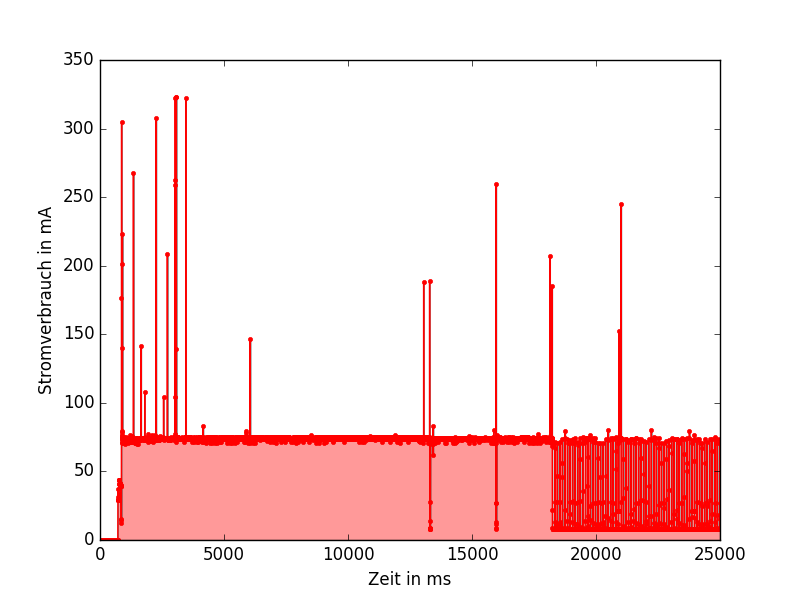
\includegraphics[width=\textwidth]{plots/radar5s.png}
  \caption{Lastkurve einer Implementierung von RADAR.}
  \label{fig:radar5s}
\end{figure}

Abbildung \ref{fig:radar5ssend} zeigt den Sendevorgang der RADAR Implementierung.
Auffällig ist, dass längerfristig empfangen wird, obwohl dies für den Versand des UDP Pakets nicht notwendig ist.\\

\begin{figure}[h!]
  \centering
	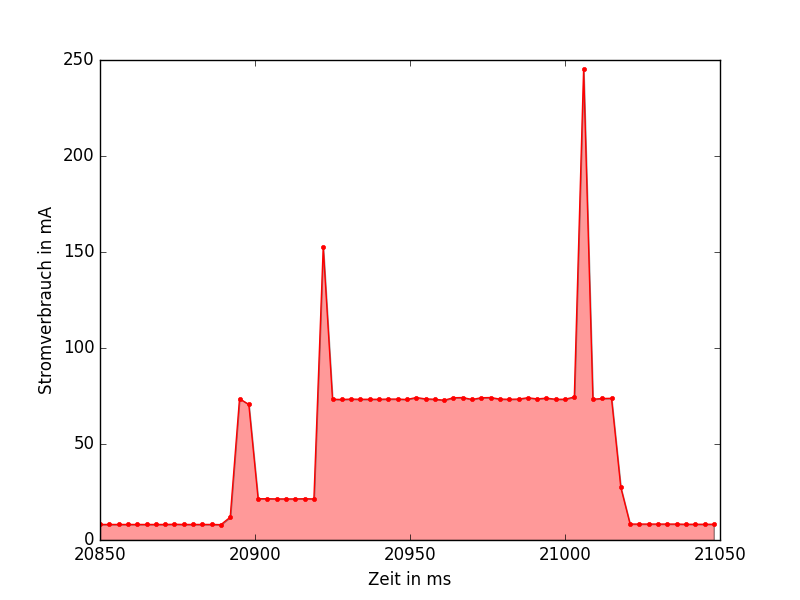
\includegraphics[width=\textwidth]{plots/radar5ssend.png}
  \caption{Lastkurve eines Ortungsvorgangs mit RADAR.}
  \label{fig:radar5ssend}
\end{figure}

In Tabelle \ref{table:radarina} ist der durchschnittliche Verbrauch der RADAR Implementierung über eine Stunde gelistet.
Es wurde sowohl mit dem ESP8266 Feather, als auch mit dem einzelnen ESP-12F gemessen, die mobile Einheit wurde jeweils erst circa eine Sekunde nach Beginn mit Strom versorgt.

\begin{table}[h!]
	\centering
	\caption{Energieverbrauch mobiler Einheiten mit RADAR Implementierung}
	\label{table:radarina}
	\begin{tabular}{p{3.5cm}|p{5cm}|p{2.5cm}|p{2.5cm}}
		Hardware & Programm & $\varnothing$ Verbrauch in mA & Laufzeit in Stunden\\
		\hline
		ESP8266 Feather & RADAR & 16,7 & 83,8\\
		ESP-12F & RADAR & 10,1 & 138,6\\
	\end{tabular}
\end{table}

\subsection{Probe Request Lokalisierung}
\label{ch:phase2:sec:powerprobereq}
Abbildung \ref{fig:probereqv} zeigt den Lastverlauf für einen Sendevorgang der Probe Request Implementierung, der Verlauf für den ESP8266 Feather ist in Rot und der Verlauf für das ESP-12F Modul ist in Grün dargestellt.\\
Nachdem der ESP8266 aus dem \texttt{deep\_sleep} erwacht beginnt eine circa 100ms andauerne Startphase, danach sendet er die drei Probe Requests.
Anschließend soll der ESP8266 wieder in den \texttt{deep\_sleep} versetzt werden, vorher empfängt er jedoch noch 100ms.
Die restliche Zeit befindet sich der ESP8266 im Tiefschlaf. 
Bei dem ESP-12F Modul ist der INA219 nicht in der Lage einen Vebrauch zu messen, er liegt unter 0,1 Milliamper.\\

\begin{figure}[h!]
  \centering
	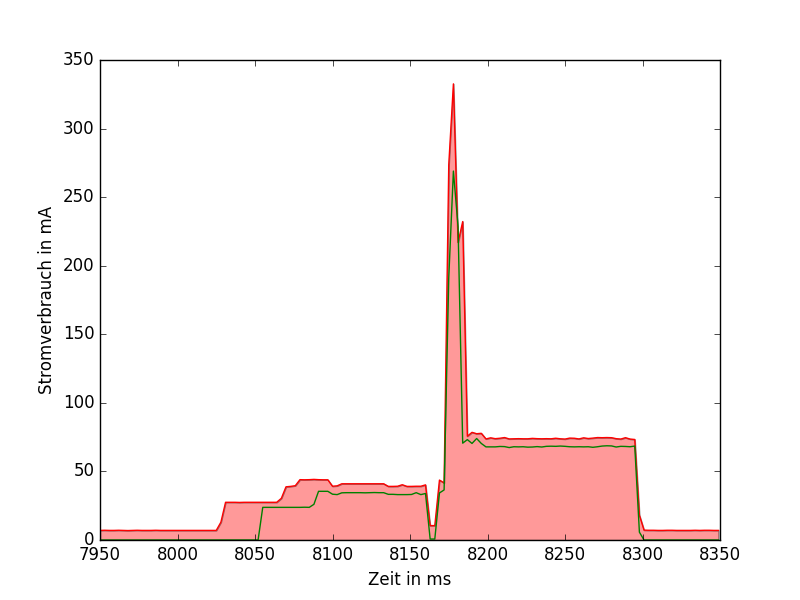
\includegraphics[width=\textwidth]{plots/probereqv.png}
  \caption{Lastkurve eines Ortungsvorgangs mit Probe Requests.}
  \label{fig:probereqv}
\end{figure}

Beim ESP8266 Feather misst er jedoch durchgehend einen Vebrauch von über 7 Milliamper, daraus ergeben sich die Unterschiede in den Messungen, die in Tabelle \ref{table:probereqina} dargestellt werden.
Es wurde sowohl mit nur einem versendeten Probe Request, als auch mit drei Probe Requests getestet, die Unterschiede im Verbrauch liegen jedoch im Bereich der Messungenauigkeit.

\begin{table}[h!]
	\centering
	\caption{Energieverbrauch mobiler Einheiten mit Probe Request Ortung}
	\label{table:probereqina}
	\begin{tabular}{p{3.5cm}|p{5cm}|p{2.5cm}|p{2.5cm}}
		Hardware & Programm & $\varnothing$ Verbrauch in mA & Laufzeit in Stunden\\
		\hline
		ESP8266 Feather & Probe Request drei Kanäle & 9,72 & 144\\
		ESP-12F & Probe Request drei Kanäle & 1,8 & 777,8\\
		ESP8266 Feather & Probe Request ein Kanal & 9,74 & 143,7\\
		ESP-12F & Probe Request ein Kanal & 1,82 & 769,2\\
	\end{tabular}
\end{table}
